
%----------------------------------------------------------------------------------------
%	PACKAGES AND OTHER DOCUMENT CONFIGURATIONS
%----------------------------------------------------------------------------------------

\documentclass[11pt]{formatting/format} % Default font size, values from 8-12pt are recommended
\usepackage{fontawesome}
\usepackage{xspace}
\usepackage{graphicx}
\graphicspath{ {./formatting/} }
%----------------------------------------------------------------------------------------

\begin{document}


\begin{minipage}[t]{0.25\textwidth} % % of the page width for name
	\vspace{-\baselineskip} % Required for vertically aligning minipages
	
	\colorbox{illustration}{{\huge\textcolor{background}{\textbf{\MakeUppercase{Oliwia}}}}} % First name
	
	\colorbox{illustration}{{\huge\textcolor{background}{\textbf{\MakeUppercase{Słupska}}}}} % Last name
	
	\vspace{6pt}
	
\end{minipage}
\begin{minipage}[t]{0.50\textwidth} % % of the page width for the first row of icons
	\vspace{-\baselineskip} % Required for vertically aligning minipages
	
	% The first parameter is the FontAwesome icon name, the second is the box size and the third is the text
 
	\icon{MapMarker}{12}{ Stockholm, Sweden }\\ \\
    \icon{LinkedinSquare}{12}{\href{https://www.linkedin.com/in/oliwia-słupska-857aa8177}{ \color{illustration} MyLinkedIn}}\\ \\
	\icon{Phone}{12}{+48 887 338 085}\\ \\
	\icon{At}{12}{\href{mailto:oliwiaslupska@gmail.com}{\color{illustration} oliwiaslupska@gmail.com}}\\
 
\end{minipage}
\begin{minipage}[t]{0.25\textwidth} % 27.5% of the page width for the second row of icons
	\vspace{-\baselineskip} % Required for vertically aligning minipages
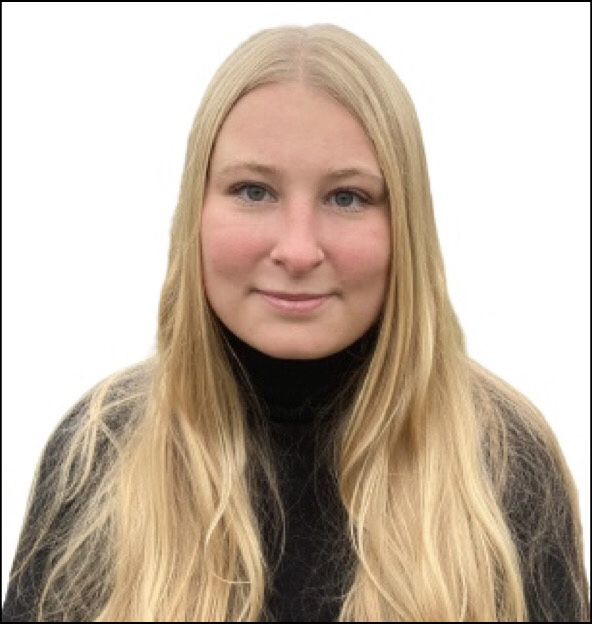
\includegraphics[scale=0.17]{photo_cv_oli}

\end{minipage}



%----------------------------------------------------------------------------------------
%	INTRODUCTION, SKILLS AND TECHNOLOGIES
%----------------------------------------------------------------------------------------
\cvsect{Who Am I?}

\begin{minipage}[t]{1\textwidth} % interchangable text space allocationk, current : 100%
	\vspace{-\baselineskip} % Required for vertically aligning minipages
	
	\color{text}{ I am a Polish graduate professional with a background in Spanish studies, translations and customer care in multinational companies. I am a language enthusiast, I have always looked for opportunities to improve my language skills. I am a people-oriented, dependable person with good problem solving skills that likes to work in multicultural environments. }
 
\end{minipage}
\hfill % Whitespace between


%----------------------------------------------------------------------------------------
%	EXPERIENCE
%----------------------------------------------------------------------------------------

\cvsect{Professional Experience}

\begin{entrylist}
	\entry
		{\color{text}}
		{\color{text} \Large Spanish Customer Service Associate  }
		{\color{text} \large 09/2022  - Now }
		{\color{text}  \large Accenture \\\\
 \normalsize As part of Accenture, I currently work for a client that is a medical device company. I take care of incoming inquiries from hospitals and clinics in Spain regarding medical equipment. My team processes the orders from our client, which come from hospitals and technicians located mainly in \textbf{Spain}. We take care of authorization of orders, changing data in \textbf{SAP and SNOW}, creating Price Quotations, as well as taking care of contact with clients, \textbf{both by email and phone}.We process the orders in SAP and Service Now and we authorize the request for technicians so that  equipment can be repaired and sent back to hospitals as quickly as possible. 
 
\begin{itemize}
\item \textbf{Answering client queries by phone and email.}
\item \textbf{Validating of contractual agreements related to Service and repair process.}
\item \textbf{Ensuring resolution of queries within the contractual metrics.}
\item \textbf{Training and supervision of new employees.} \\
\end{itemize}
 }
	\entry
		{\color{text} }
		{\color{text} \Large Programme Coordinator, English Teacher }
		{\large   06/2017 - 09/2022}
		{\color{text} \large Angloville \\\\
   \normalsize Teaching English to adults on weekend courses, conducting classes and individual language sessions at English camps for children aged 12-19, being a leading coordinator for English programmes of  \textbf{60} people (40 participants and 20 English native speakers from around the World) in Poland, Malta, Greece, England and other european countries.
  \begin{itemize} \item \normalsize \textbf{Leading and organizing learning programmes.}
 \item \textbf{Designing Dashboards on Tableau} to have interactive monitoring of treasury.
 \item \textbf{Cooperating with the head office, hotels and native speaker
coordinators. } 
 \item \textbf{Database management. } 
 \item \textbf{Training and supervision of new employees.} 
 \item \textbf{Providing support to young people away from home on English camps.}\\
  \end{itemize}
  }
  \entry
		{\color{text} }
		{\color{text} \Large Library Manager }
		{\large   11/2018 - 06/2019}
		{\color{text} \large Cerventes Institute \\\
   \normalsize 
  \begin{itemize} \item \normalsize \textbf{Providing Customer service}:  Guiding teachers to find the best materials for their lessons, building a trusted relationship with clients from Spain, Latin America and Poland   
 \item \textbf{Operating systems and database of the Institute} : Updating and cleaning database with SQL.
 \item \textbf{Performing business translations from Spanish to Polish/English.}
 \item \textbf{Database management.} 
 \\
  \end{itemize}
  }
\end{entrylist}
 

%----------------------------------------------------------------------------------------
%	EDUCATION
%----------------------------------------------------------------------------------------
\cvsect{Education}
\begin{entrylist}
    \entry
        {\color{text} }
        {\color{text} \Large Master Degree in Applied Linguistics}
        {\color{text} \large 10/2020 - Now}
        {\color{text} \large University of Warsaw \\  
         \begin{itemize}
       \item \normalsize  My studies allowed me to improve two languages, Spanish and English. I gained knowledge in economics, business, medicine, law, science and technology, literature, linguistics, literary studies and many others and mastered the vocabulary needed to translate in these areas. I have also gained technical knowledge that has enabled me to operate CAT tools, subtitling programmes and master HTML.\\
        \end{itemize}}

    \entry
        {\color{text} }
        {\color{text} \Large Master Degree in Translation and Interpreting}
        {\color{text} \large 09/2021 - 03/2022}
        {\color{text} \large The Autonomous University of Barcelona \\  
         \begin{itemize}
       \item \normalsize  Studying in Barcelona allowed me to get to know the Spanish culture, experience education in an international environment and master skills in translations and
interpreting.\\
        \end{itemize}}

    \entry
        {\color{text} }
        {\color{text} \Large Bachelor degree in Spanish and Iberian Studies}
        {\color{text} \large 10/2016 - 07/2020}
        {\color{text} \large SWPS University} \\    
\end{entrylist}

\cvsect{Languages}

\color{text}\textbf{Polish }  - C2 Native \\
\color{text}\textbf{English}  - C1 Fluent \\
\color{text}\textbf{Spanish}  - C1 Fluent \\
\color{text}\textbf{Swedish} - A2  \\
%----------------------------------------------------------------------------------------
%	Skills
%----------------------------------------------------------------------------------------

\cvsect{Skills}
\color{text}\textbf{Personal skills} : {Excellent interpersonal skills and time management, deep understanding of client's need, data analytic, excellent communication, attention to details. }\\

\color{text}\textbf{Tools} : HTML, CAT Tools, Excel, MySQL, SAP R3 \& S4 , Service Now, Tableau, TeX language.



%----------------------------------------------------------------------------------------
%	HOBBIES 
%----------------------------------------------------------------------------------------

\cvsect{Hobbies \&  interest}
\\
\small\textbf{Animal Rescue, Cinema, Outdoors, Books, Traveling, History of Art, Cooking}  


\begin{center} 
\color{text}\footnotesize\ -- LaTeX code of this resume can be found \color{illustration}\href{https://github.com/DGloi/TexResumeTemplate}{here} \color{text} -\end{center}



%----------------------------------------------------------------------------------------
\end{document}
